\chapter{Science with ILC}
%\writer{Keisuke Fujii}{2}

Our ultimate goal is to achieve a unified understanding of nature, which is to go back in time to the moment of creation, when everything, matter, force, and space-time, is thought to be unified. One way to study the early universe is to observe distant space with telescopes. This method, however, cannot penetrate into the very early universe before formation of hydrogen atoms, i.e. 380 thousand years after the Big Bang (the recombination epoch), when the Universe was still opaque to light. Energy frontier collider experiments provide a unique opportunity to investigate the universe before the recombination by reproducing in a controlled manner reactions that could happen only in the very early universe. Our current understanding of the early universe on a microscopic scale is summarised in the Standard Model (SM) of particle physics. The SM consists of matter fermions (quarks and leptons), force carrying vector bosons (gauge bosons), and a scalar boson (Higgs boson) designed specifically to give masses, where needed, to otherwise massless SM particles by breaking the electroweak symmetry through Higgs condensation in the vacuum. The 2012 discovery of the Higgs boson at the LHC has completed the SM particle spectrum. 

Up to now, the SM has survived all the intense scrutiny searches for new particles at energy frontier colliders such as LEP, Tevatron, and, most recently, the LHC, through precision measurements of the $W$ and $Z$ bosons, and through searches for anomalies in flavor physics. While being extremely successful, however, the SM has left many open questions such as what is the nature of dark matter and dark energy,  why matter, not antimatter, dominates the universe, what is the origin of neutrino masses and mixings, and why did the Higgs field fill the entire universe and why at the electroweak scale. These questions call for physics beyond the Standard Model (BSM). The Higgs boson discovery hence marked the start of a new voyage to the moment of creation.

The ILC is going to explore uncharted waters at and beyond the electroweak scale, i.e. about one trillionth of a second after the Big Bang, in order to directly address the question: why did the Higgs field fill the entire Universe and why did it do so at the electroweak scale. 
The Higgs boson is at the center of this question, which makes precision Higgs study of utmost importance. The ILC will fully exploit the Higgs boson as a new tool to discover BSM physics responsible for the mystery of the electroweak scale.
%Since the Higgs boson discovery, the LHC has so far seen no new particle or phenomenon, indicating that existing techniques to look for BSM physics at existing particle physics facilities are approaching their limits. 
%This makes precision Higgs study of utmost importance. The ILC is going to fully exploit the Higgs boson as a new discovery tool and will explore the energies at and beyond the electroweak scale, in order to directly address the question: why did the Higgs field fill the entire Universe and why at the electroweak scale, i.e. about one trillionth of a second after the Bing Bang. 

A key observable is precision measurements of Higgs couplings to various SM particles. In the SM the Higgs boson's couplings to various SM particles are proportional to their masses. BSM physics modifies this proportionality, leaving its nature (existence of another dimension, or a deeper stratum of matter, or multi-verse?) imprinted in the deviation pattern from the SM. 
% as in Fig.\,\ref{fig:DeviationPatterns}. 
%\begin{figure}[htbp]
%\begin{center}
% 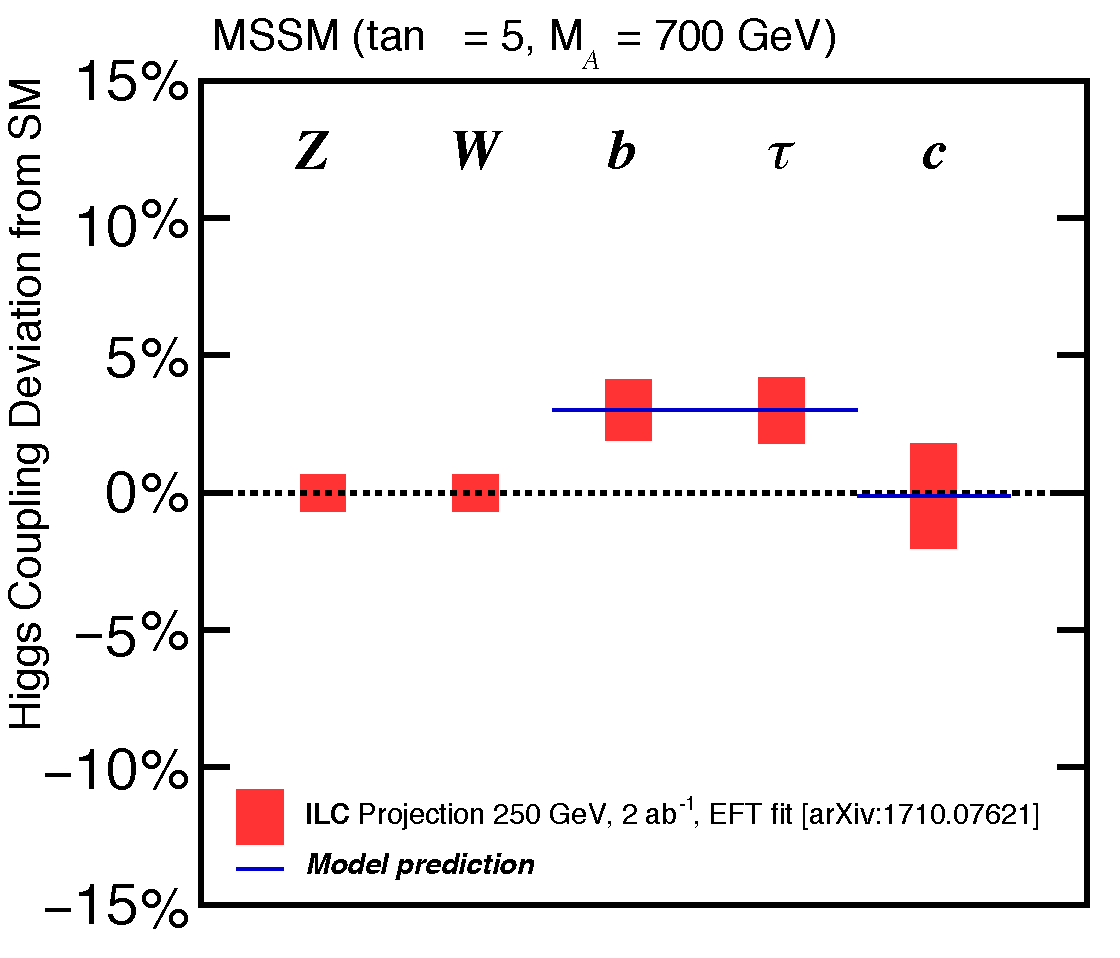
\includegraphics[width=0.3\textwidth]{Science/fig/PatternMSSM.pdf}\hspace{2mm}
% 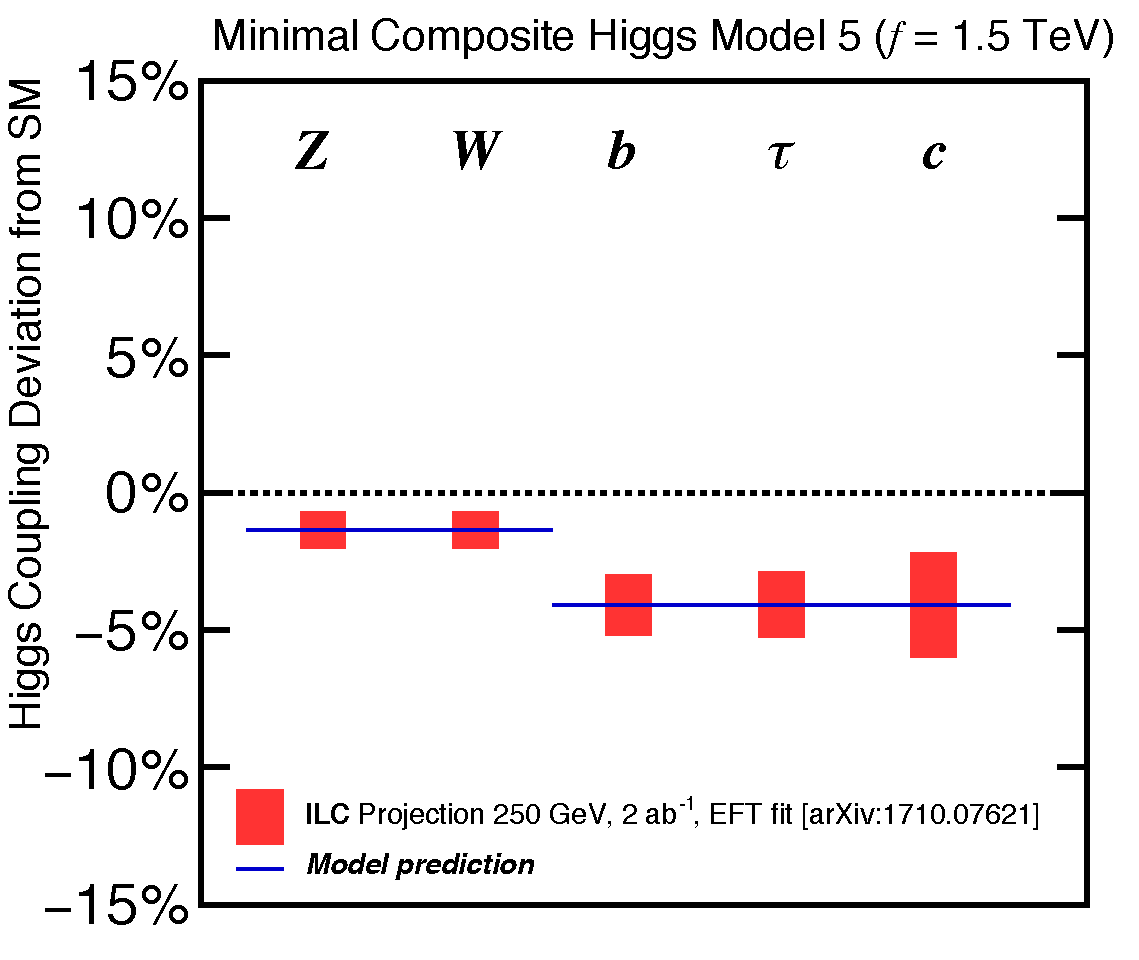
\includegraphics[width=0.3\textwidth]{Science/fig/PatternComposite.pdf}\hspace{2mm}
% 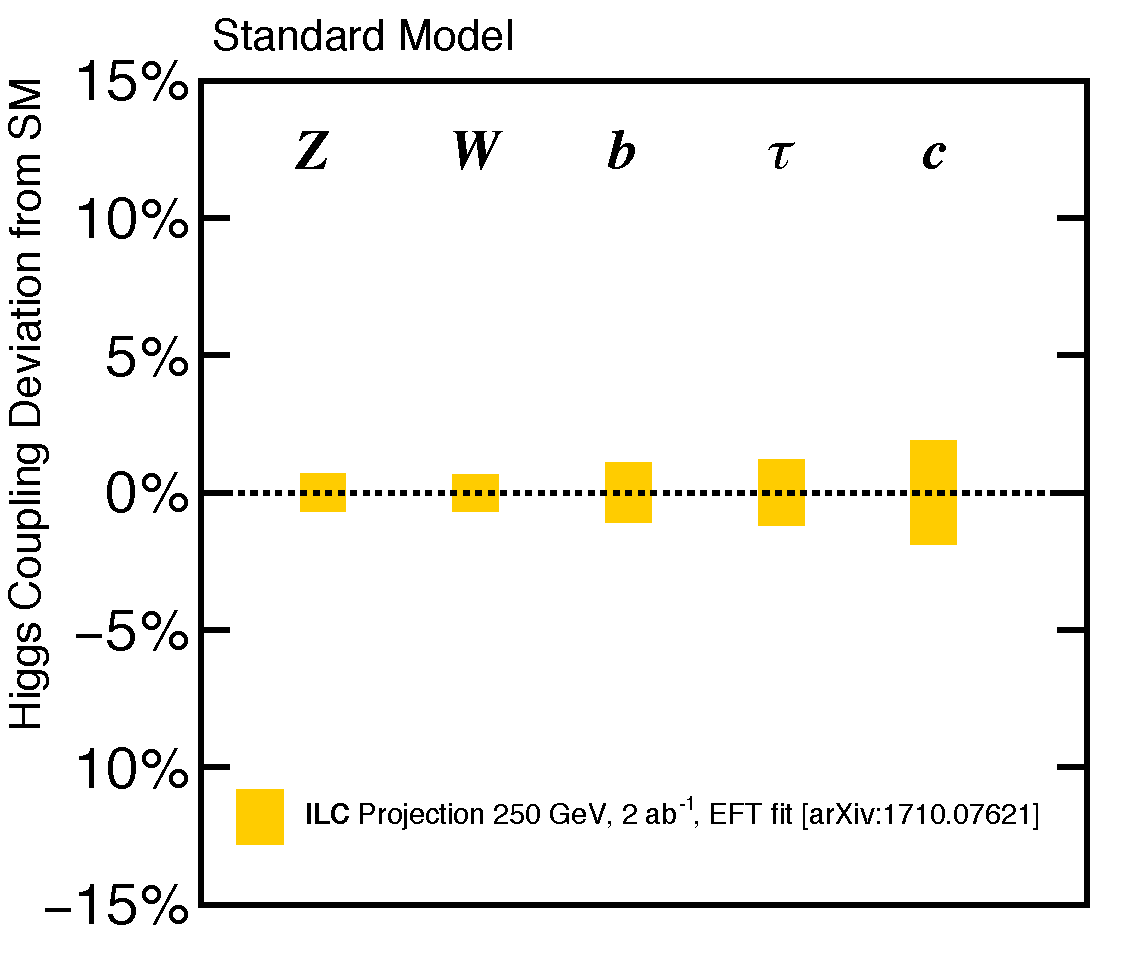
\includegraphics[width=0.3\textwidth]{Science/fig/PatternSM.pdf}
%\end{center}
%\caption{Typical deviation patterns for SUSY (left), Composite Higgs (centre), and SM (right).
%}
%\label{fig:DeviationPatterns}
%\end{figure}
%There are three possibilities. The first is the road of another dimension, supersymmetry (SUSY) or extra-dimension, where the Higgs boson is elementary. This road leads us directly to the ultimate unification. The second is the road of deeper stratum of matter, where the Higgs boson is composite, implying the existence of new strong force and many composite particles in the multi-TeV region. The third is the road where the SM, as it is, holds up to a very high scale. This road requires a new principle, such as the existence of multiverse. 
%
%

The ATLAS and CMS experiments at the LHC have measured the Higgs couplings to the vector bosons and the third generation matter fermions and found them consistent with the SM predictions within errors at the 10\,\% level~\cite{Cepeda:2019klc}. The HL-LHC is expected to significantly improve the measurement accuracies to a 2-4\,\% level~\cite{Ref:HL-LHC}. These accuracies would be, however, insufficient, since expected deviations are typically at a level of 5\.\% or smaller due to the famous decoupling theorem~\cite{Ref:Decoupling}. To see the deviations and their pattern and to decide the future direction of particle physics, we need a percent level precision for various Higgs couplings.

% [Design Concept = to reconstruction events at the "parton" level]
The primary goal of the ILD experiment is to measure various Higgs couplings to a \% level or better, so as to make a decisive step in deciphering the physics beyond the Standard Model, and to help to 
decide the future direction of particle physics from their deviation pattern. ILD is also to measure properties of the $W$ and $Z$ bosons and fermion pair production with unprecedented precision, while searching directly for new particles with unprecedented sensitivity, in order to further elucidate new physics that lies beyond the electroweak scale.

% [Design Principle = PFA, hermeticity, flavor ID]
To achieve this goal, the ILD experiment has to reach a new level of precision in the reconstruction of final states. It aims at reconstructing every event at the level of quarks, leptons, and fundamental bosons including gauge bosons and the Higgs boson, so as to see events as if viewing a Feynman diagrams. For this purpose, the ILD design has been optimized for Particle Flow Analysis (PFA), enforced by precision vertexing to tag heavy flavors and hermeticity to indirectly detect invisible particles such as neutrinos and dark matter particles. 
% [Design Principle = usable up to 1 TeV]

To benefit maximally from the energy upgradability of the ILC machine, ILD has been designed to be an experiment at a collider providing electron-positron collisions at centre-of-mass energies between 90\,GeV and about 1\,TeV, which allows a broad and long-term physics program that will evolve depending on the results from earlier stages. New particle searches at higher energies guided by a specific deviation pattern of Higgs couplings found at 250\,GeV are a typical case of such evolution. There is, however, a set of guaranteed physics of crucial importance at higher energy stages. The top quark, which is the heaviest in the SM and hence expected to be tightly coupled to the electroweak symmetry breaking sector, will enter our physics program at $\sqrt{s} \gtrsim 350$\,GeV. The 500\.GeV stage allows us to directly access the top Yukawa coupling through $t\bar{t}H$ production and the triple Higgs coupling through $ZHH$ production. The measurement precision for the top Yukawa and the triple Higgs couplings will be significantly improved at 1\,TeV. An up-to-date presentation of the physics case of the ILC project can be found in
\cite{ILCESU1}.
%
%The science goals of the ILC have been described in detail in \cite{ILCESU1}.
%The physics program using electron positron collisions will enable us to take a new and different look at the physics of the Standard Model, and in particular, at probing the boundaries of the validity of the Standard Model. 
%Up to now, we have sought evidence for new interactions or new particles from direct searches for new particles at LEP, the Tevatron, and, most recently, the LHC, from measurements of the $W$ and $Z$ bosons, and from searches for anomalies in flavor physics.  We are now approaching the limits of these techniques with current particle physics facilities.  The ILC will extend our search capabilities in precision measurements of $W$ boson couplings and fermion pair production, and will provide new opportunities for the direct discovery of new particles.  But, most of all, it will open a completely new road through the  high-precision study of the Higgs boson. 
%Indeed, the core physics program at the ILC is to make high-precision measurements of the properties of the Higgs boson, for a range of different centre-of-mass energies. 
% The Higgs-boson is playing a central role in the Standard Model. Since its discovery at the LHC, a first determination of its properties has taken place, but many open questions remain. 
%Many of the key properties of the Higgs boson are currently known only to the 10\% level. With the ILC, it will be possible to improve most of these errors to the 1\% level or below, to a point where the quantities become sensitive to radiative corrections. %In this way, knowing precisely the properties of the Higgs not only tells us about the least well-known particle in the Standard Model, but also provides an entry point into physics and science beyond the Higgs and beyond the Standard Model. 
%This approach has a great potential to contribute to the study and understanding of natures in areas where the standard model clearly is not enough.  It cannot for example address basic facts about the universe in the large, in particular, the excess of matter over antimatter and the origin of the cosmic dark matter. To make progress, we need observational evidence from particle physics of violations of the SM.  These will provide clues that can show the way forward.
\\

In the context of the ILD group a broad range of studies have been undertaken to understand the potential of the ILD experiment at the ILC up to 1\,TeV. 
%A very brief summary of the main results will be given in the remainder of this chapter. 
It is important to point out that these studies are based on fully simulated events, using a realistic detector model and advanced reconstruction software, and in many cases include estimates of major systematic effects. This is particularly important when estimating the physics reach the ILC and ILD will have for specific measurements. Determining, for example, the branching ratios of the Higgs boson at the percent level depends critically on the detector performance, and thus on the quality of the event simulation and reconstruction.
It should also be emphasized that, in many cases, the performance used in the physics analyses has been tested against prototype experiments. The performance numbers decisive for vertexing, tracking, and calorimetry are all based on results from test beam experiments. These test beam results include those regarding single particle resolution for neutral and charged particles, particle separation in jets, one-to-one linking power between charged tracks and calorimeter clusters, and many aspects of detailed shower analyses. The PFA performance, a crucial element that decides the ILD physics reach, has been corroborated by these test beam results, though its full demonstration has to wait for a larger scale test beam experiment that combines these major detector aspects. 
A very brief summary of the main results from the ILD full simulation studies will be given in the remainder of this chapter.
\\

%[Recoil mass]
One of the most important Higgs measurements at the ILC is that of the $e^+e^- \to ZH$ process with the recoil mass technique, which allows us to measure the total $ZH$ production cross section ($\sigma_{ZH}$) decay-mode-independently and hence to absolutely normalize Higgs couplings. This is in contrast to measurements at the LHC, where initial state 4-momenta of colliding partons are unknown and hence the recoil mass technique cannot be applied. Figure \ref{fig:Mhrecoilmm} (left) shows the mass distribution of the system recoiling against the $\mu^+\mu^-$ pair from a $Z$ decay\cite{Yan:2016xyx}. We can see a clear Higgs peak sticking out from the background without looking at the decay products of the Higgs boson. This way we will be able to determine the Higgs boson mass to $14$\,MeV with $2\,{\rm ab}^{-1}$ at $\sqrt{s}=250$\,GeV.
\begin{figure}[htbp]
\begin{center}
 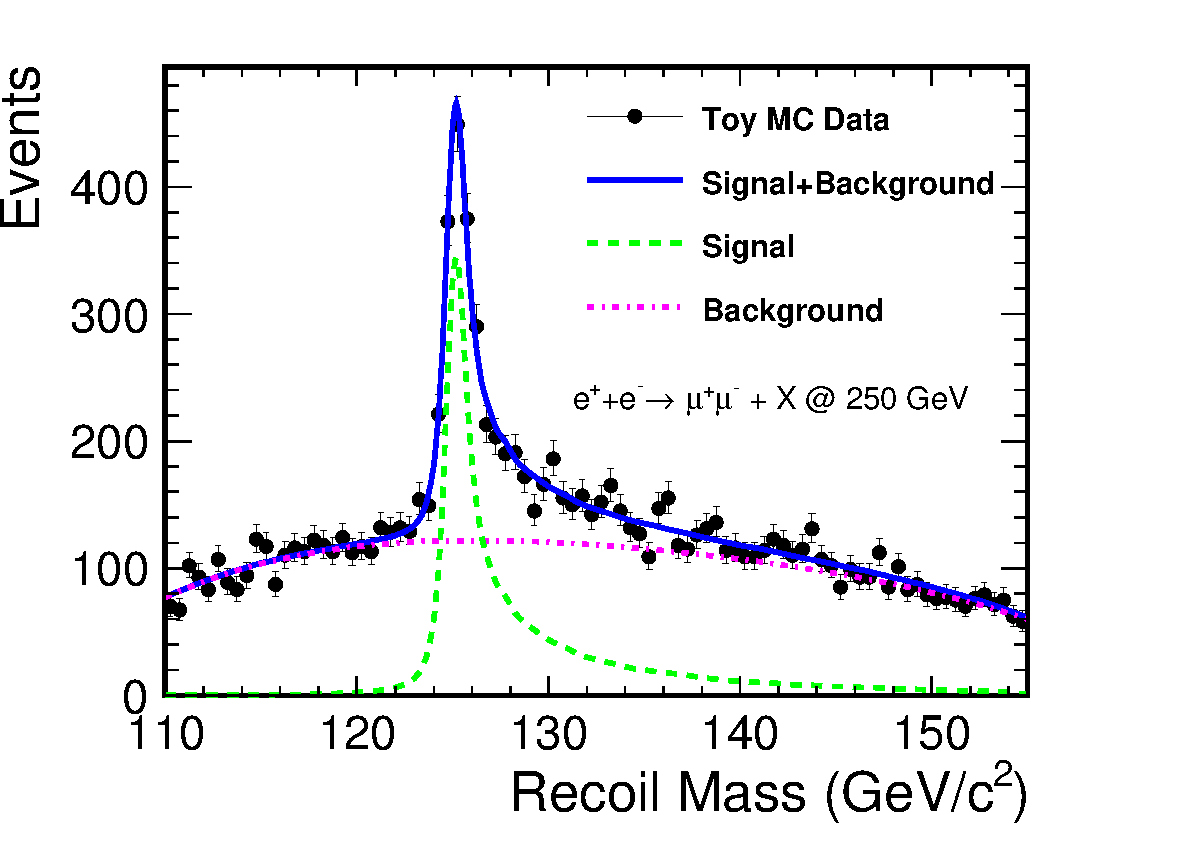
\includegraphics[width=0.48\textwidth]{Science/fig/RecoilMassLep250.pdf}\hspace{2mm}
 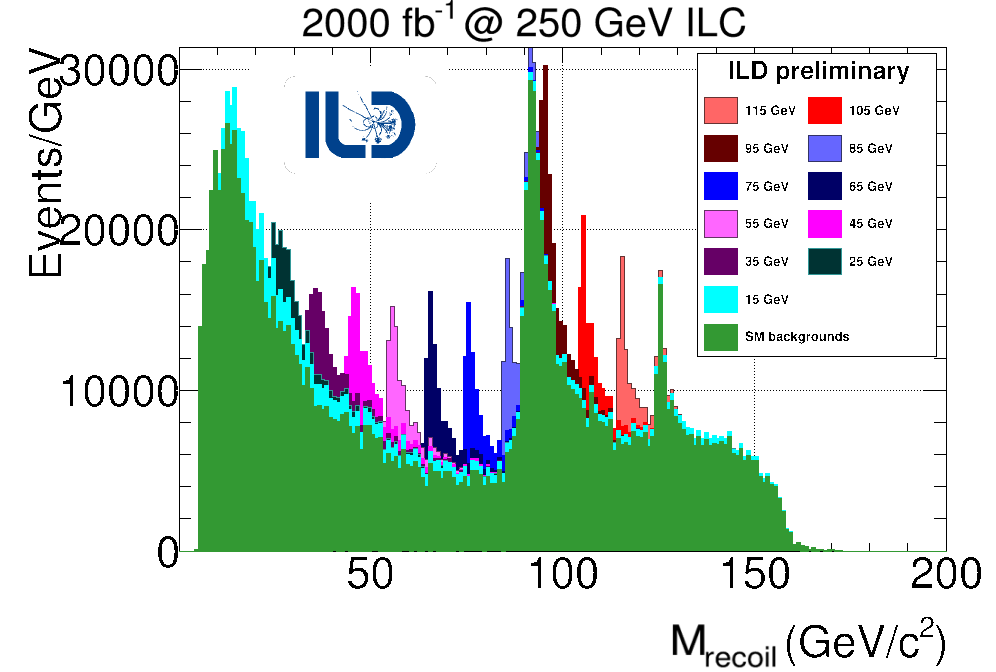
\includegraphics[width=0.48\textwidth]{Science/fig/po_muon_kcut_recoil_mass_summary1.png}
\end{center}
\caption{Recoil mass distribution for $e^+e^- \to ZH$ followed by a $Z \to \mu^+\mu^-$ decay at $\sqrt{s}=250\,$GeV (left). A plot similar to the left figure but with an additional scalar particle recoiling against the Z boson (right). 
}
\label{fig:Mhrecoilmm}
\end{figure}
With the same integrated luminosity, by combining the $Z \to e^+e^-$ and $Z \to q\bar{q}$ channels, we can measure the absolutely normalized $\sigma_{ZH}$ to 2.0\% for both $e^-_Le^+_R$ and $e^-_Re^+_L$ beam polarisations.  
The same technique can be used to search for a new scalar boson or the Higgs to dark matter decays.
Figure\,\ref{fig:Mhrecoilmm} (right) shows expected recoil-mass peaks of additional scalar bosons having the same coupling to $Z$ as the SM Higgs boson but with various different masses. 
%This analysis is detailed in [Section\,$8.3.10$]. 
Notice that a high momentum resolution as from the ILD tracking is essential to see these sharp peaks with their widths limited not by the detector resolution but only by the beam energy spread. For the search for the invisible Higgs decays, we take advantage of the higher branching ratio for hadronic $Z$ decays. With the 2\,ab$^{-1}$ at $\sqrt{s}=250$\,GeV, ILD will be able to put a 95\,\%C.L. upper limit of 0.3\,\% on $BR(H\to \mathrm{invisible})$\cite{Ref:Hinvisible}.
% (see [Section\,8.3.4] for a similar analysis at 500\,GeV).
%

The $\sigma_{ZH}$ measured with the recoil mass technique is used to extract the branching ratio of the Higgs boson to a pair of SM particles ($X$) from its corresponding $\sigma_{ZH} \times BR(H \to XX)$ measurement. Here the ILC's clean environment and ILD's excellent flavor tagging capability play a central role to separate $H \to c\bar{c}$ and $H \to gg$ decays, not to mention the dominant $H \to b{bar}$ decay.
% (see [Section\,$8.3.1$]). 
While the direct detection of the $H \to c\bar{c}$ and $H \to gg$ decays is challenging at the LHC, the LHC can measure the ratios of branching ratios in high precision for decay modes with small branching ratios as long as they have clean signatures. For a Higgs decay such as $H \to \gamma\gamma$ which has a branching ratio of a per-mille level, its measurement at the ILC alone will be statistics-limited. The combination of the measurement of the ratio, $BR(H \to \gamma\gamma)/BR(H \to ZZ^*)$ at the LHC and that of  $BR(H \to ZZ^*)$ at the ILC allows the measurement of the $H\to\gamma\gamma$ coupling to 1\,\%, which is a typical example of LHC-ILC synergy.

%[Manhattan plot]
In order to extract an absolutely normalized Higgs coupling, $g_{HXX}$, from the corresponding measured branching ratio, $BR(H \to XX)$, we need to know the total width, $\Gamma_H$, of the Higgs boson. The total width is, however, only 4\.MeV in the SM, which is too small for a direct measurement. The most recent method to overcome this difficulty and to determine the Higgs couplings is to perform a global fit in the framework of the SM Effective Field Theory (SMEFT)\cite{Barklow:2017suo,Barklow:2017awn}. The SMEFT framework links observables directly involving the Higgs boson to those without the Higgs boson, through the $SU(2) \times U(1)$ gauge symmetry. This allows us to make full use of all the measurements with ILD, not only those directly involving the Higgs boson, but all the others regarding precision electroweak observables or processes without the Higgs boson such as $e^+e^ \to W^+W^-$\cite{Karl:2019hes}. The beam polarizations play a crucial role here to lift degeneracies between different EFT operators and to control systematic uncertainties. Figure\,\ref{fig:Manhattan} shows the projected precision of various Higgs couplings from the SMEFT fit for the 250\,GeV ILC (green) and its upgrade to 500\,GeV (blue), where the lighter bands assume some future improvements in ILC measurements\cite{ILCESU1}.
%%%%
\begin{figure}[htbp]
\begin{center}
 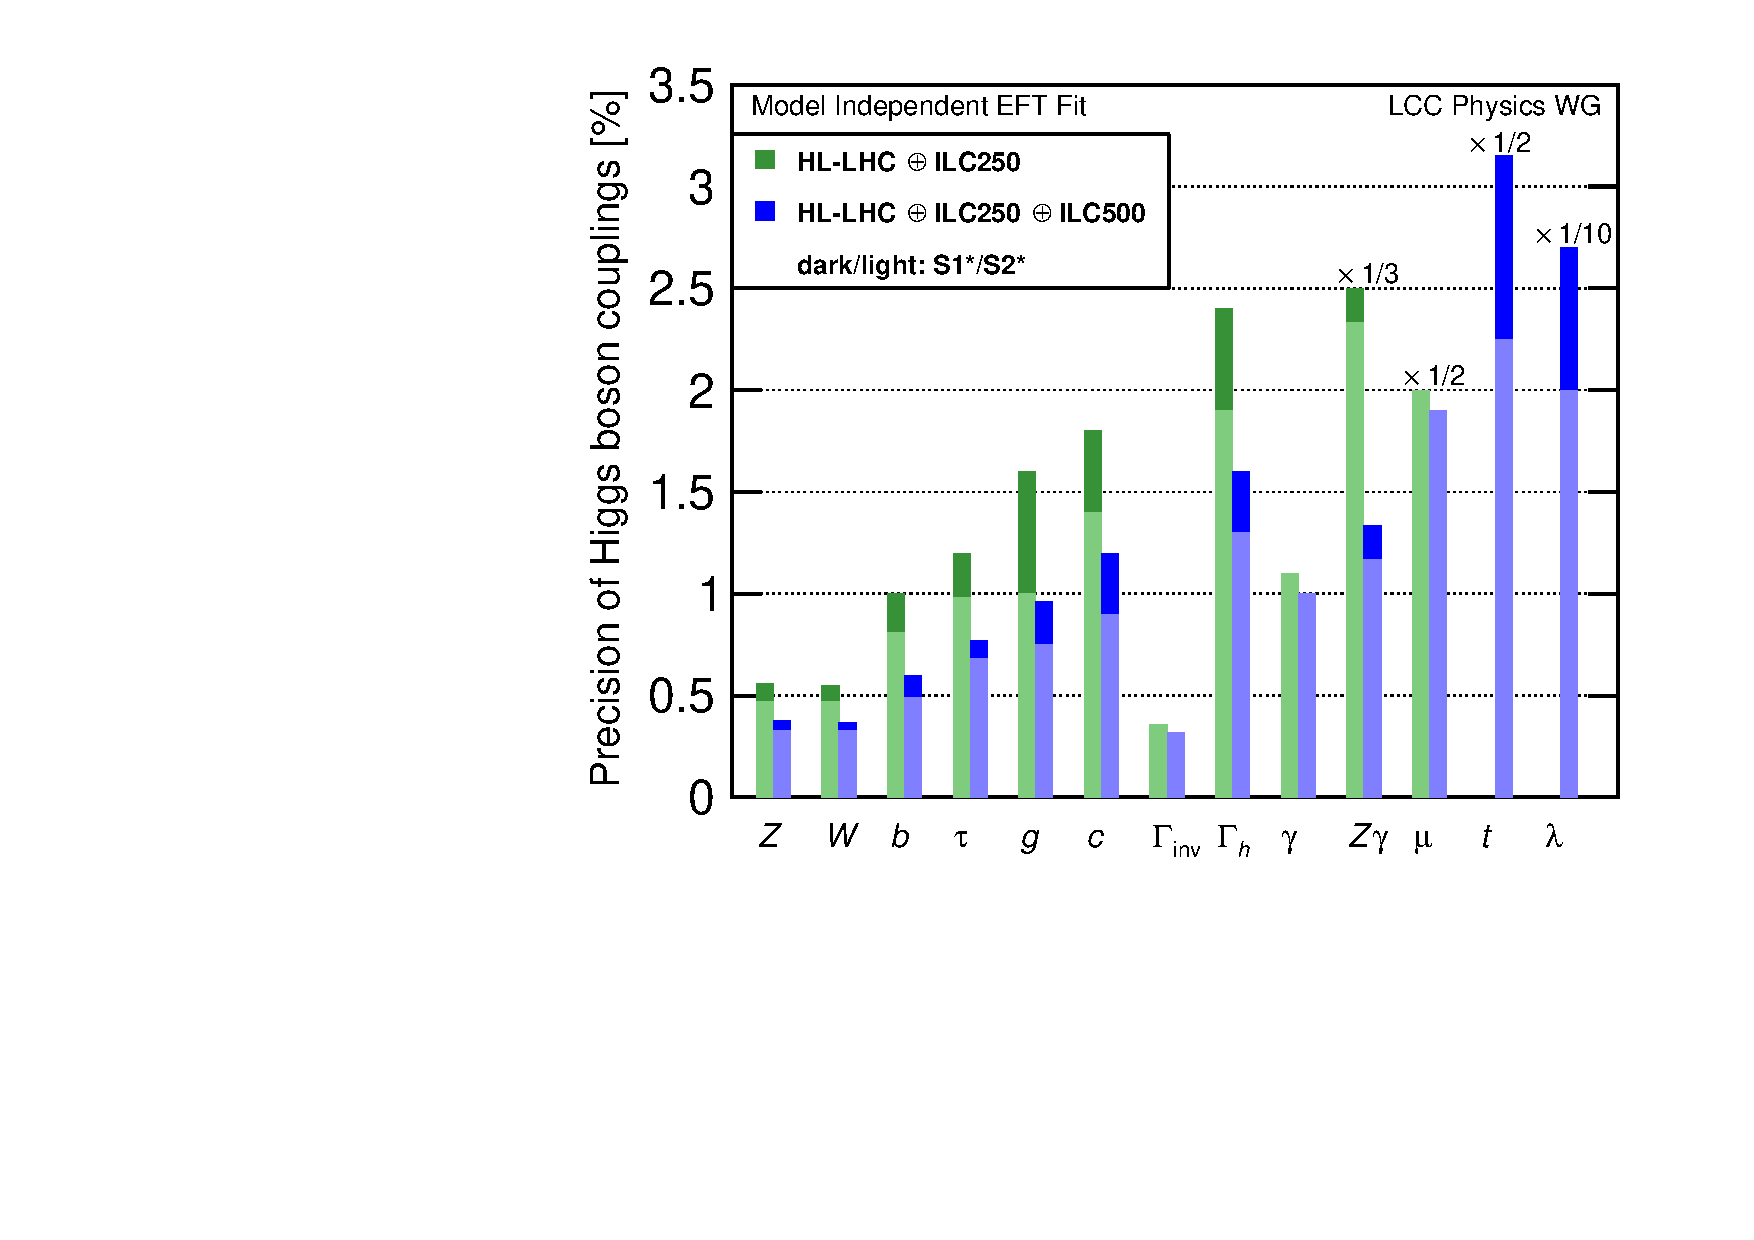
\includegraphics[width=0.5\textwidth]{Science/fig/DeltaHXX_SM_ILC_MI_S12s.pdf}
\end{center}
\caption{Projected precisions of Higgs boson couplings from the SMEFT fit for the 250\,GeV ILC (green) and its upgrade to 500\,GeV (blue), where the lighter bands assume some future improvements in ILC measurements\cite{ILCESU1}.
}
\label{fig:Manhattan}
\end{figure}
%%%%
We can see that, already at 250\,GeV, the precisions reach the target level of 1\,\% for most of the major couplings, which will be significantly improved at 500\,GeV.
%
% [We might insert traffic signal plots here.]
%

%[Mono-photons]: hermeticity
We have seen above how the ILD experiment will enable us to achieve the ILC's primary goal as a Higgs factory. The ILC is, however, not only a Higgs factory but also a new particle discovery machine. Notice here the following four points that enhance sensitivities to regions with small cross sections and compressed mass spectra, which are challenging at the LHC. First, the ILC's integrated luminosity at 250\,GeV is $10^3$ times more than that collected by 4 LEP experiments together at the highest energies. Second, the ILD detector is much more advanced than LEP detectors thanks to the advance in detector technologies since the LEP time. Third, the ILC provides polarised beams, a very powerful tool to control signal and background processes. Finally, the ILC's beam structure allows trigger-less data taking. The search for WIMP pair production is one of the most important targets of new particle searches both at the LHC and the ILC. The LHC has a mass reach much higher than the ILC. Nevertheless, there will be a significant fraction of WIMP parameter space left unexplored even after the HL-LHC. The yellow area in Fig.\,\ref{fig:WIMPleft} is such regions remaining after searches at the (HL-)LHC as well as current or future direct detection experiments\cite{Habermehl:2017dxh}.
\begin{figure}[htbp]
\begin{center}
 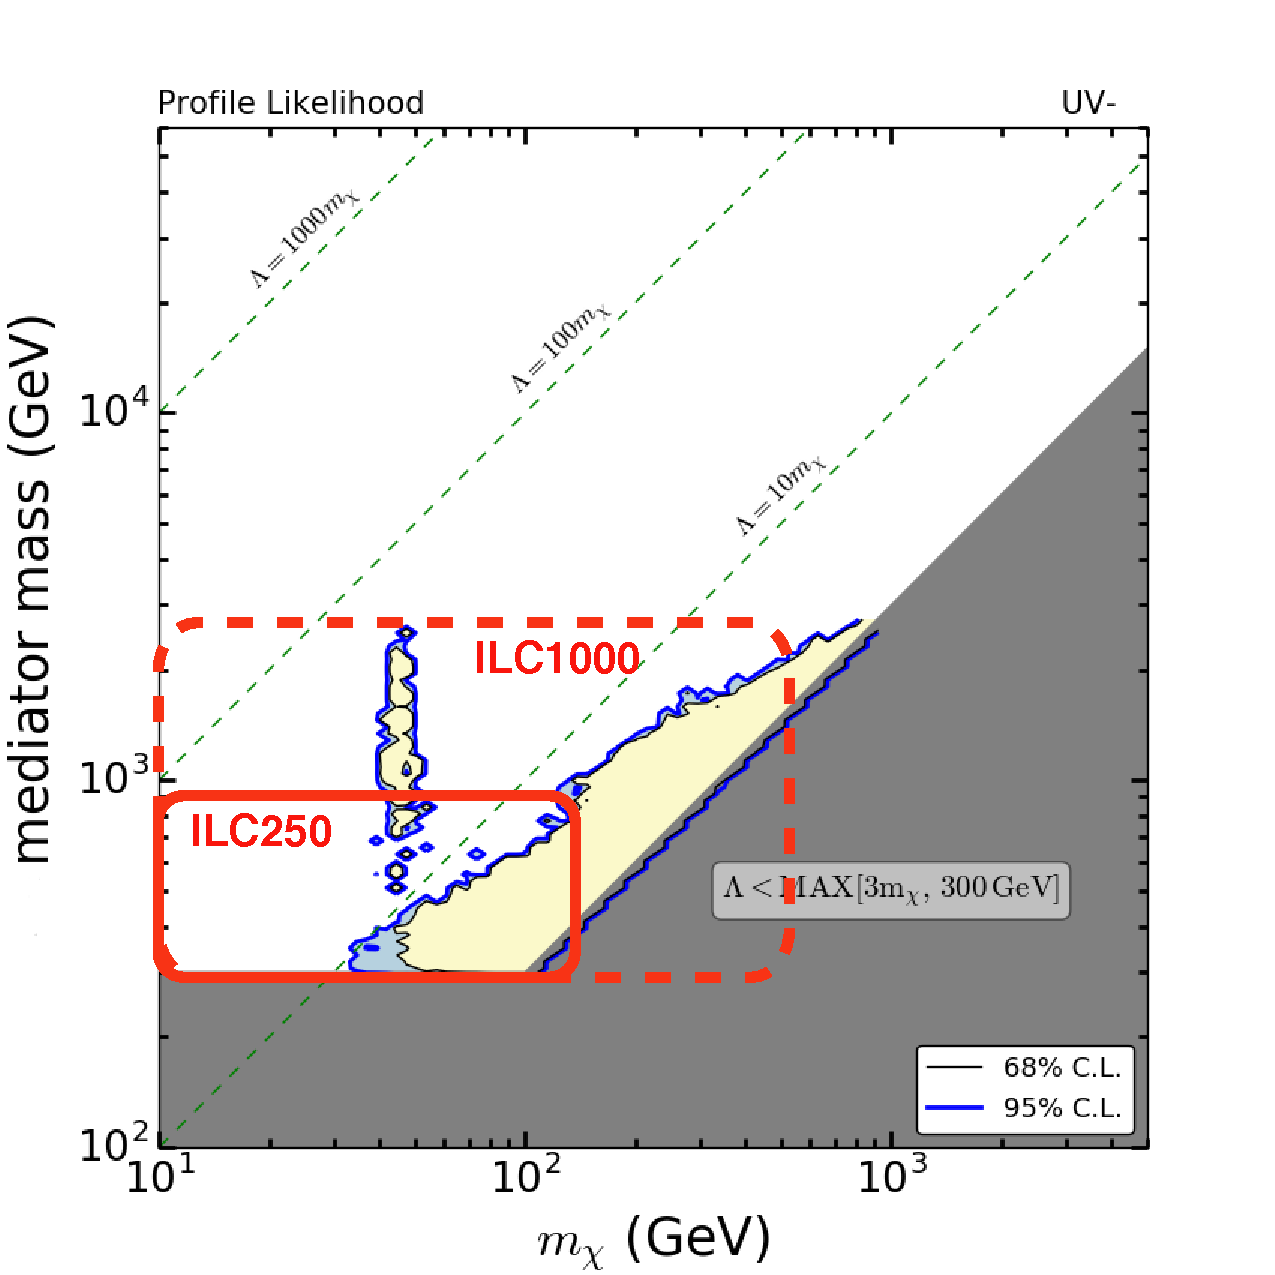
\includegraphics[width=0.5\textwidth]{Science/fig/UVminus_mx_lam_far_2ilc.pdf}
\end{center}
\caption{Portion of WIMP parameter space (yellow area) expected to survive searches at the (HL-)LHC as well as current and future direct searches. The solid and dashed red boxes indicate, respectively, the regions the 250\,GeV ILC and its 1\,TeV upgrade will be sensitive to\cite{Ref:ilcWIMP}.
}
\label{fig:ilcWIMP}
\end{figure}
The red solid box indicates the region the 250\,GeV ILC will probe, which is already substantial. The 1\,TeV upgrade will expand the ILC's sensitivity to the red dashed box covering a large fraction of the remaining WIMP parameter space\cite{Ref:ilcWIMP}. In addition to the beam polarisations, the excellent calorimetric coverage of the ILD detector, hermetic down to about 5\,mrad to the beam axes, is essential to veto Bhabha background so as to achieve this high sensitivity. 
%The mono-photon search at the ILC is detailed in [Section\,8.3.12].

%[Higgsinos]: loop-hole free searches
A search for higgsinos is another example for which detection is challenging at the LHC because of their compressed mass spectrum. Such higgsinos are expected to be light and their mass differences typically below 20\,GeV in the natural SUSY models, while the other SUSY particles may be beyond the reach of even the HL-LHC. As demonstrated in \cite{Baer:2016new}, ILD can not only discover such higgsinos but also measure their masses and production cross sections, which can be used, together with the Higgs-related measurements described above, in a global fit to extract underlying SUSY model parameters, which in turn provides an opportunity to test high scale physics such as gaugino mass unification and various SUSY breaking scenarios. Here again, the ILD's high sensitivity to higgsinos with small mass differences are due to the hermeticity of the ILD detector and its excellent tracking capability over a wide momentum range.

%[Top] with dE/dx
As already mentioned, the top quark, being the heaviest in the SM, might hold the key to the mystery of the electroweak symmetry breaking. Its measurement starts in the 350\,GeV stage of the ILC at around the $t\bar{t}$ threshold. The $t\bar{t}$ threshold provides an ideal laboratory to measure a short-distance top quark mass such as $m_t(\bar{\mathrm MS})$. With ILD we can measure $m_t(\bar{\mathrm MS})$ to 50\,MeV\cite{Horiguchi:2013wra, Vos:2016ti} and, together with the aforementioned Higgs mass measurement, test stability of the SM vacuum. 

In the 500\,GeV stage, our main focus of top quark physics will shift to form factor measurements for the top quark couplings to the photon and the $Z$ boson. Partially composite top quarks, which often accrue from composite Higgs models, are to modify the $t\bar{t}Z$ form factors and cause significant deviations from the SM expectations with characteristic deviation pattern for couplings to $t_L$ and $t_R$. With ILD, we can determine these form factors separately to accuracies better than 0.3\%
%(see [Section\,8.3.9]) 
by measuring the cross section and forward-backward asymmetry for the $t\bar{t}$ pair production with 4\,ab$^{-1}$ at 500\,GeV\cite{Amjad:2015mma}. 
Figure\,\ref{fig:ttZ_gLgR} compares the expected ILD precision for 500\,fb$^{-1}$ with various BSM models.
\begin{figure}[htbp]
\begin{center}
 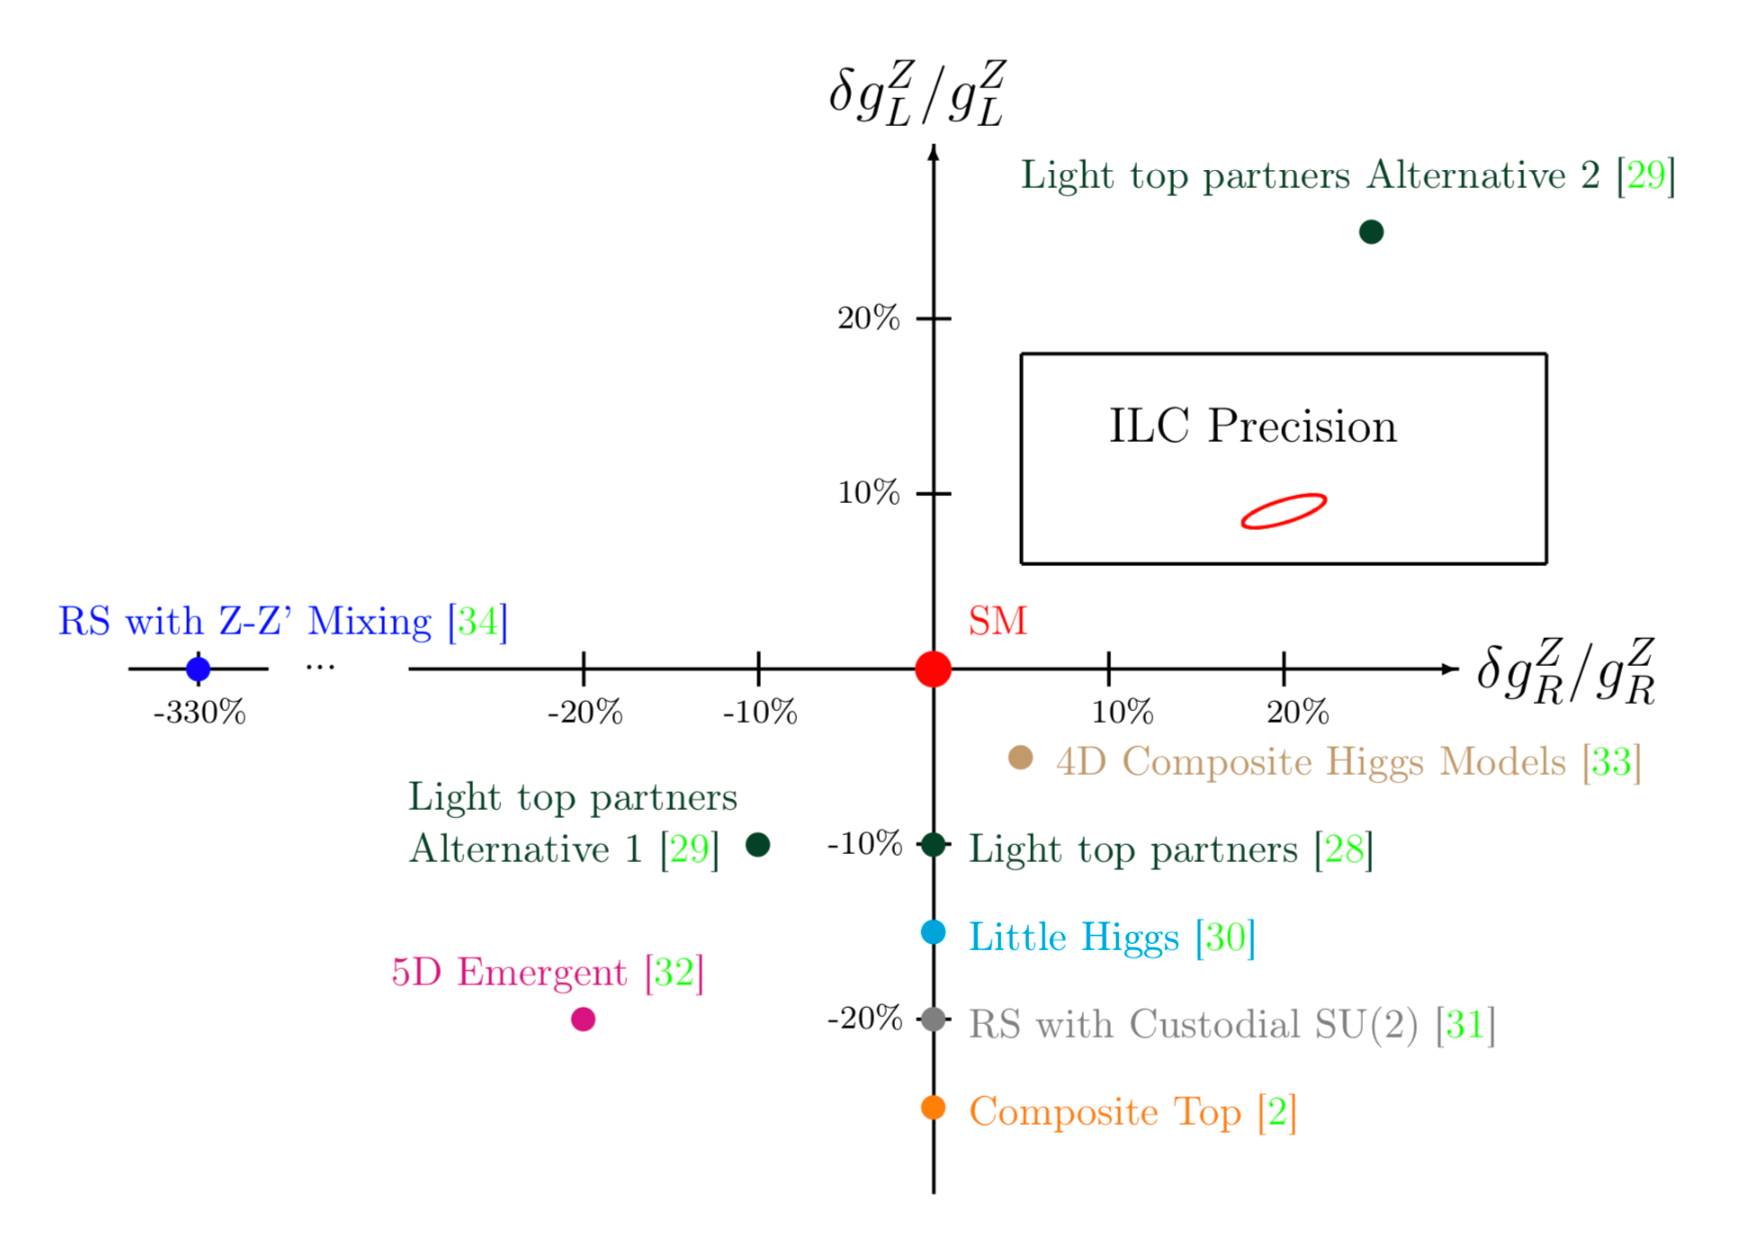
\includegraphics[width=0.6\textwidth]{Science/fig/ttZ_gLgR}
\end{center}
\caption{Expected deviations of the $t_L$ and $t_R$ couplings to the $Z$ boson for various BSM models compared with the expected ILC precision for 500\,fb$^{-1}$ at 500\,GeV\cite{Ref:FttZ}.
}
\label{fig:ttZ_gLgR}
\end{figure}
The form factor measurements will hence give us yet another handle to elucidate BSM physics responsible for the electroweak symmetry breaking, in addition to the precision Higgs measurements described above. It should be emphasized that combination of vertex charge and the Kaon ID using $dE/dx$ information from the ILD TPC plays a substantial role in the forward-backward asymmetry measurement of the $t\bar{t}$ production.
\\

%[WW scattering]: PFA
%The longitudinal components of the $W$ and $Z$ bosons stem from the Higgs sector. If the deviation pattern of the  Higgs couplings indicates compositeness of the Higgs boson in particular, the importance of measuring high energy $WW$ and $ZZ$ scattering processes would be significantly enhanced, for which separation of the $WW$ and the $ZZ$ final states is crucial. ILD performed a full simulation study of these processes at $\sqrt{s}=1$\,TeV and demonstrated that hadronic decays of $W$ and $Z$ bosons can be cleanly separated thanks to the excellent PFA performance\cite{Ref:VVscattering}. 
%The same analysis is revisited in [Section\,8.3.6] with more realism including full overlay of $\gamma\gamma \to$ low-$p_t$ hadrons and $e^+e^-$ pair background.
%
% Ref:VVscattering, 



While the physics case studies are based on the version of the ILD detector presented in the detector volume of the ILC DBD~\cite{Behnke:2013lya}, ILD has recently initiated a systematic bench-marking effort to study the performance of the ILD concept, and to determine in particular the correlations between science objectives and detector performance. The list of benchmark analyses which are under study is given in table \ref{tab-benchmark}. 
Notice also that, although the ILC will start operation at the centre-of-mass energy of 250\,GeV, the ILD detector is being designed to meet more challenging requirements at higher centre-of-mass energies, since major parts of the detector, e.g.\ the coil, the yoke and the main calorimeters will not be replaced when upgrading the accelerator. Therefore, most of the detector benchmark analyses are performed at the centre-of-mass energy of 500\,GeV, and one benchmark even at 1\,TeV. The assumed integrated luminosities and beam polarisation settings follow the canonical running scenario~\cite{Barklow:2015tja}. 
In addition to the well-established performance aspects of the ILD detector, the potential of new features not yet incorporated in the existing detector prototypes, e.g.\ time-of-flight information, is being evaluated.\\

%\begin{comment}
\begin{table}[thb]
    \centering
    \begin{tabular}{|p{4cm}|p{5cm}|p {5cm}|}
\hline
{\bf    Measurement}     & {\bf Main physics question} & {\bf main issue addressed} \\
\hline
Higgs mass in $H\rightarrow b {\bar b}$         &  Precision Higgs mass determination &Flavour tag, jet energy resolution, lepton momentum resolution  \\
\hline
Branching ratio $H \rightarrow \mu^+\mu^-$ & Rare decay, Higgs Yukawa coupling to muons & High-momentum $p_t$ resolution, $\mu$ identification \\
\hline
Limit on $H \rightarrow$ invisible & Hidden sector / Higgs portal & Jet energy resolution, $Z$ or recoil mass resolution, hermeticity\\
\hline
Coupling between Z and left-handed $\tau$ & Contact interactions, new physics related to 3rd generation & Highly boosted topologies, $\tau$ reconstruction, $\pi^0$ reconstruction \\
\hline
$WW$ production, $W$ mass & Anomalous triple gauge couplings, $W$ mass&  Jet energy resolution, leptons in forward direction \\
\hline
Cross section of $e^+e^- \rightarrow \nu \nu qqqq$ & Vector Bosons Scattering, test validity of SM at high energies&  $W/Z$ separation, jet energy resolution, hermeticity\\
\hline
Left-Right asymmetry in $e^+e^- \rightarrow \gamma Z$ & Full dim-6 EFT interpretation of Higgs measurements &  Jet energy scale calibration, lepton and photon reconstruction \\
\hline
Hadronic branching ratios for $H\rightarrow b \bar b $ and $c \bar c$ & New physics modifying the Higgs couplings &  Flavour tag, jet energy resolution\\

\hline
$A_{FB}, A_{LR}$ from $e^+e^- \to b\bar{b}$ and $t \bar t \rightarrow b\bar{b} qqqq / b \bar{b} qql\nu$ & Form factors, electroweak coupling &  Flavour tag, PID, (multi-)jet final states with jet and vertex charge\\
\hline

Discovery range for low $\Delta M$ Higgsinos & Testing SUSY in an area inaccessible for the LHC& Tracks with very low $p_t$, ISR photon identification, finding multiple vertices\\
\hline
Discovery range for WIMP's in mono-photon channel & Invisible particles, Dark sector & Photon detection at all angles, tagging power in the very forward calorimeters\\
\hline
Discovery range for extra Higgs bosons in $e^+e^- \rightarrow Zh$ & Additional scalars with reduced couplings to the $Z$ & Isolated muon finding, ISR photon identification.\\
\hline

%\hline
%\multicolumn{3}{|l|}{Running above the top threshold:}\\


    \end{tabular}
    \caption{Table of benchmark reactions which are used by ILD to optimize the detector performance. The analyses are mostly conducted at 500\,GeV centre-of-mass energy, to optimally study the detector sensitivty. The channel, the physics motivation, and the main detector performance parameters are given.}
    \label{tab-benchmark}
\end{table}
%\end{comment}

%==========
% References
%==========
%
% Ref:LHCHiggs, 
% Ref:HL-LHC, M. Cepeda et al. (Physics of the HL-LHC Working Group), (2019), arXiv:1902.00134 [hep-ph].
% Ref:Decoupling, H. E. Haber, in Joint U.S.-Polish Workshop on Physics from Planck Scale to Electro-Weak Scale (SUSY 94) Warsaw, Poland, September 21-24, 1994 (1994) pp. 1\UTF{2013} 16, [,1(1994)], arXiv:hep-ph/9501320 [hep-ph].

% Ref:Hrecoil, J. Yan, S. Watanuki, K. Fujii, A. Ishikawa, D. Jeans, J. Strube, J. Tian, and H. Yamamoto, Phys. Rev. D94, 113002 (2016), arXiv:1604.07524 [hep-ex].
% Ref:Hinvisible, A. Ishikawa, “Search for invisible higgs decays at the ilc,” presentation at Linear Collider Work- shop, Belgrade, Serbia, October 5-10, 2014, http://agenda.linearcollider.org/event/6389/ session/0/contribution/140 (2014).

% Ref:EFT1, T. Barklow, K. Fujii, S. Jung, R. Karl, J. List, T. Ogawa, M. E. Peskin, and J. Tian, Phys. Rev. D97, 053003 (2018), arXiv:1708.08912 [hep-ph].
% Ref:EFT2, T. Barklow, K. Fujii, S. Jung, M. E. Peskin, and J. Tian, Phys. Rev. D97, 053004 (2018), arXiv:1708.09079 [hep-ph].
% Ref:WW, R. Karl, From the Machine-Detector Interface to Electroweak Precision Measurements at the ILC — Beam Gas Backgrounds, Beam Polarization and Triple Gauge Couplings, Dissertation, Universitat Hamburg, Hamburg (2019), DESY-THESIS-2019-018.

% Ref:ilcWIMP, M. Habermehl, K. Fujii, J. List, S. Matsumoto and T. Tanabe, PoS ICHEP 2016, 155 (2016) [arXiv:1702.05377 [hep-ex]].

% Ref:Higgsino, H. Baer, M. Berggren, K. Fujii, S.-L. Lehtinen, J. List, T. Tanabe, and J. Yan, Proceedings, 38th Interna- tional Conference on High Energy Physics (ICHEP 2016): Chicago, IL, USA, August 3-10, 2016, PoS ICHEP2016, 156 (2016), arXiv:1611.02846 [hep-ph].

%
% Ref:ttbarThreshold, T. Horiguchi, A. Ishikawa, T. Suehara, K. Fujii, Y. Sumino, Y. Kiyo, and H. Yamamoto, (2013), arXiv:1310.0563 [hep-ex].
% Ref:top2016, M. Vos et al., (2016), arXiv:1604.08122 [hep-ex].
% Ref:FttZ, M. S. Amjad et al., Eur. Phys. J. C75, 512 (2015), arXiv:1505.06020 [hep-ex].



